\documentclass{article}

\oddsidemargin=0in
\evensidemargin=0in
\textwidth=6in
\topmargin=0in
\textheight=9in

\parindent=0in
\pagestyle{empty}

\usepackage{amsfonts}
\usepackage{amssymb}
\usepackage[pdftex]{graphicx}




\begin{document}

\section*{Chapter 1:  Explanation of the Algorithm} 
 \noindent The problem which needs to be solved is as follows: there are a number of objects, which all have a size and a value, and we have a knapsack which has a capacity. This means that it only can take a certain amount of objects. These objects should amount to a value that is as large as possible.\\

\begin{figure}[h!]
  \centering
    \reflectbox{%
      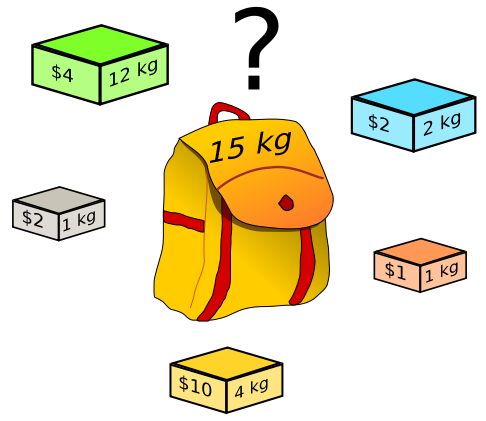
\includegraphics[width=0.5\textwidth]{Knapsack.png}}
  \caption{An illustration of the Knapsack problem!}
\end{figure}





\textbf{Elementary operation:} We are counting the number of objects that are in the input file defined as n, and the number of possible subsets which can be created from them ($2^n$), defined as m.\\

\noindent \textbf{Pseudocode:}
\begin{tabbing}
For \= all the objects in the input file \\
\> create \= all possible subsets	\\
\> select the best subset with the highest value\\
\end{tabbing}

The algorithm exists of three parts. First when reading the input file each of these objects is put into a Tuple which has a size and a value. Secondly, the algorithm creates all possible subsets of the input Tuples, and the third step of the algorithm is to select the best subset, which is desirably equal to the capacity of the knapsack and has the highest value. \\
 


\section*{Chapter 2: Algorithm in Pseudocode}

\noindent The following is the pseudocode for the function "createPowerset()". \newline
%just to show how to write this in latex
for i $\rightarrow 2^n$


%Before creating sets, the program reads the input file which specifies a certain amount of items, each item is put into a Tuple, which has a size and a value. The tuple is then saved in an ArrayList. As a next step the algorithm creates a power set, where the possible number of tuple combinations are $2^n$. Through bit masking and the logical bitwise "and" operator, it is checked if the corresponding bits are both 1, in which case the current tuple is saved in a temporary array list and with help of the shift left operator $<<$ the element is shifted one step to the left. 


\section*{Chapter 3: Correctness Justification}

\section*{Chapter 4: Complexity Analysis}

\section*{Chapter 5: Performance Test}

\end{document}
